\documentclass[dvipdfmx, 9pt, a4paper]{jsarticle}
\usepackage[margin=15mm]{geometry}
\usepackage{fancyhdr}
\usepackage{multirow}
\usepackage{amsmath,  amssymb}
\usepackage{type1cm}
\usepackage{latexsym}
\usepackage{algorithmic}
\usepackage{algorithm}
\usepackage{ascmac}
\usepackage{listings,jvlisting}
\usepackage{tcolorbox}
\usepackage[utf8]{inputenc}
\usepackage{color}

\DeclareFixedFont{\ttb}{T1}{txtt}{bx}{n}{9}
\DeclareFixedFont{\ttm}{T1}{txtt}{m}{n}{9}
\definecolor{deepblue}{rgb}{0,0,0.5}
\definecolor{deepred}{rgb}{0.6,0,0}
\definecolor{deepgreen}{rgb}{0,0.5,0}

\renewcommand{\baselinestretch}{0.78}
\newcommand{\bm}[1]{{\mbox{\boldmath $#1$}}}
\newtheorem{Proof}{証明}
\def\qed{\hfill $\Box$}

\newcommand\pythonstyle{\lstset{
language=Python,
basicstyle=\ttm,
morekeywords={self},
keywordstyle=\ttb\color{deepblue},
emph={MyClass,__init__},
emphstyle=\ttb\color{deepred},
stringstyle=\color{deepgreen},
frame=tb,
showstringspaces=false
}}

\lstnewenvironment{python}[1][]
{
\pythonstyle
\lstset{#1}
}
{}

\newcommand\pythonexternal[2][]{{
\pythonstyle
\lstinputlisting[#1]{#2}}}
\newcommand\pythoninline[1]{{\pythonstyle\lstinline!#1!}}


\begin{document}
\begin{center}
{\fontsize{18pt}{1pt}\selectfont 音響拡散方程式}\\
\end{center}
\section*{はじめに}
室内音響における残響音を表現する支配方程式として音響拡散方程式(Acoustic diffusion equation)が提案されている。本資料はこの支配方程式の導出と解釈の紹介を目的とした。拡散方程式には必ず拡散項と呼ばれるものが存在するが、実は音響学において拡散項を目にすることはほとんどない。輸送現象論という学問によると、拡散項は$D\Delta w$の形で書き表されるらしく、確かに線形オイラー方程式や質量保存則においてこのような項は存在しない(波動方程式やヘルムホルツ方程式では存在するが、それらの解釈は本資料の範疇を超えるので省略する)。なお、$D$は拡散係数と呼ばれるもので、$w$は拡散対象の物理量であり、原子数密度や運動量だったりする(音響拡散方程式の場合$w$は音響エネルギー密度)。\par
私の知る限りだと、拡散を加味しなければならない音響問題は音響メタマテリアルの分野である。音響メタマテリアルのような微小空間における運動量保存則では空気とメタマテリアルの摩擦が無視できなくなる。このときの支配方程式は
\begin{equation}
\partial_t\bm v+(\bm v\cdot \bm \nabla)\bm v=-\frac{1}{\rho_0}\bm \nabla p+\nu \Delta \bm v \notag
\end{equation}
となるが、このうち右辺第二項は正に拡散項の形をしている。ちなみに右辺第二項は粘性応力と呼ばれるもので、$\nu$は動粘性係数と言い、拡散係数に相当する。つまり運動量保存則における粘性応力は拡散と同意であり、私たちは前者の呼び方を基本的に使っていることになる(同様に拡散は様々な支配方程式で登場するが、支配方程式毎に別の呼び方を持っていることが多い。例えば伝熱学における拡散は熱伝導と呼ばれる。そのまま拡散という言葉を使うのはイオンや溶質の移動といった化学の分野で多い)。\par
しかしながら、繰り返しになるが室内音響然り多くの音響問題では拡散項を考えない。それにも関わらず室内音響において音響拡散方程式なるものが提案されているのは何故か。そして、そもそも拡散現象が$D\Delta w$のような形で表現できるかも私たちは分かっていない。\par
後者の質問には連続体力学が答えてくれる。ただし前者を含めた理解にはそれだけだと不十分で、統計力学の知見が必要になる。これら領域の学習をすればある程度音響拡散方程式を理解できるが、それは余りにも大変すぎる。本資料では特に統計力学の知見を意識させないような説明を心がけた(その代わり厳密さを欠いた議論になっている)。

\section{拡散現象}
\subsection{物質拡散の直感的理解}

\begin{figure}[b]
\begin{center}
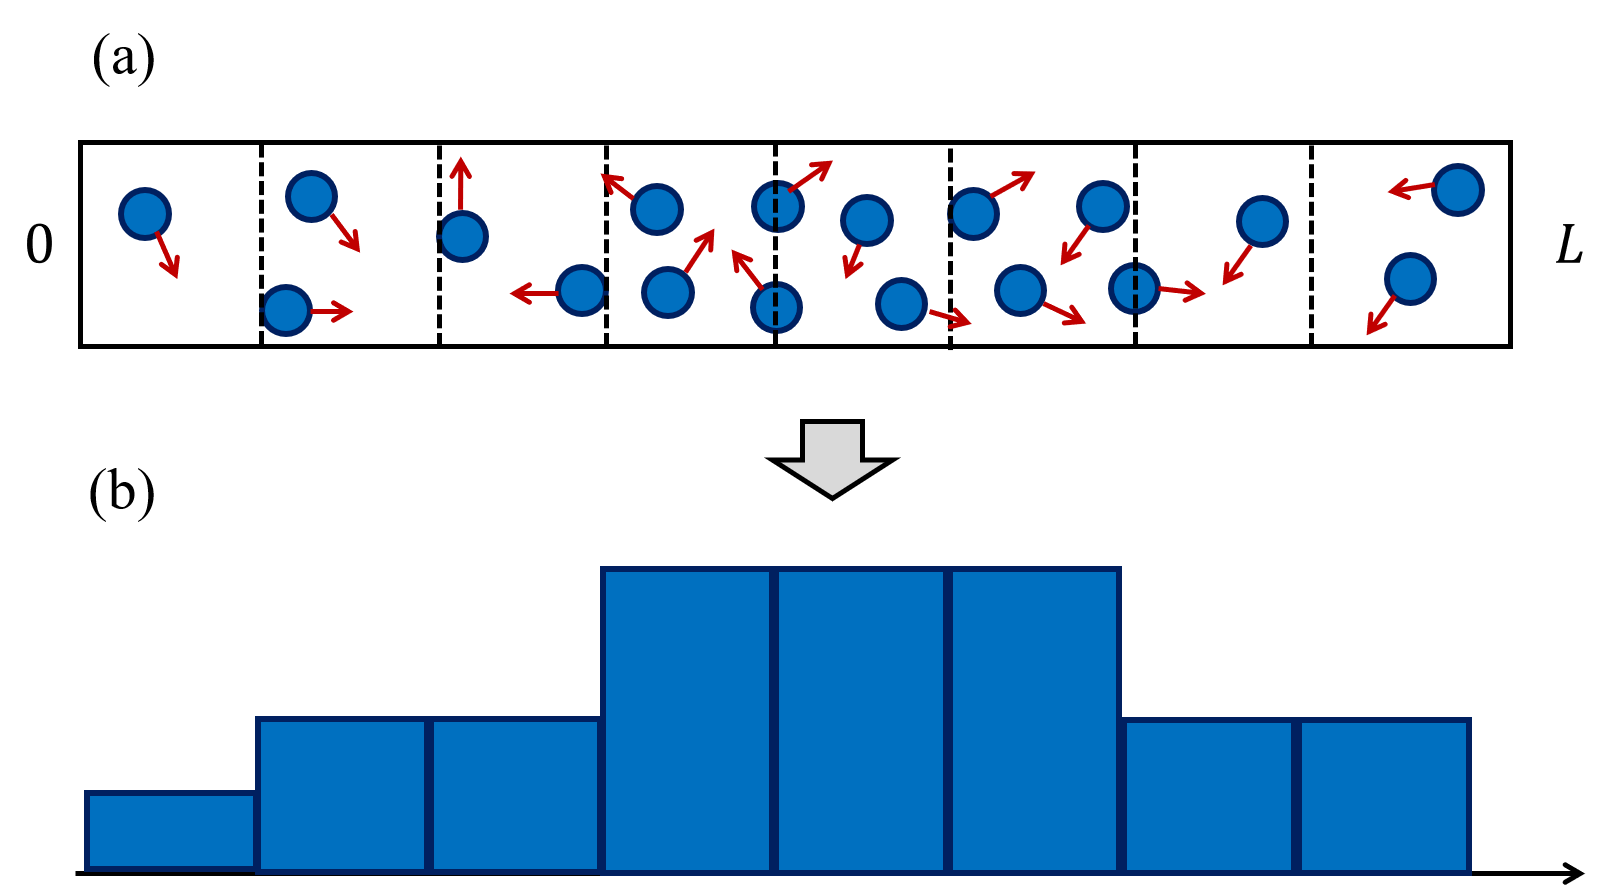
\includegraphics[width=10cm]{fig1.png}
\caption{分子の空間分布。(a)1次元空間$[0, L]$内にある分子の概念図。赤の矢印は各分子の速度ベクトル(b)離散空間分布に関するヒストグラム。}
\end{center}
\end{figure}

拡散現象の大まかな理解のために、分子の拡散から議論していく。ご存じの通り光学におけるレイトレーシングは光子の移動を追跡しており、幾何音響は類似性を確保するために音響エネルギーを有する仮想的な粒子を扱う。後述するように波動拡散方程式は仮想的な粒子群をマクロに捉えて定式化する訳だが、いきなり仮想的なものを扱うと理解が難しい。それゆえ想像のしやすい物質拡散から議論する次第である。\par
いま$[0, L]$の1次元空間内に$N$個の分子が存在しているとする(図1(a))。1次元空間をいくつかの領域に分割し、各領域に含まれる分子の数をカウントすれば、分子の離散的な空間分布が得られる(図1(b))。マクロに見たとき空間中に流れは存在しないとしても、各分子は熱的ゆらぎにより移動をしている。また分子同士の衝突により、分子の移動方向は頻繁に変化する(ブラウン運動)。統計力学ではこの運動をランダムウォークで模擬する。\par
そこで、図2(a)のような分子の初期分布を考えよう。この状態から分子をランダムウォークさせたとき、分子の空間分布は図2(b)のように時間発展していく。図2より分布の山が全体へと広がるような現象が確認できる。このような物質の輸送現象を拡散という。ご想像頂いている通り、「水の中に塩を加えたとき、塩分濃度がどのように時間発展するか」や「部屋の中の臭気源から、臭いがどのように広がっていくか」といった現象をよく表している。

\begin{figure}[t]
\begin{center}
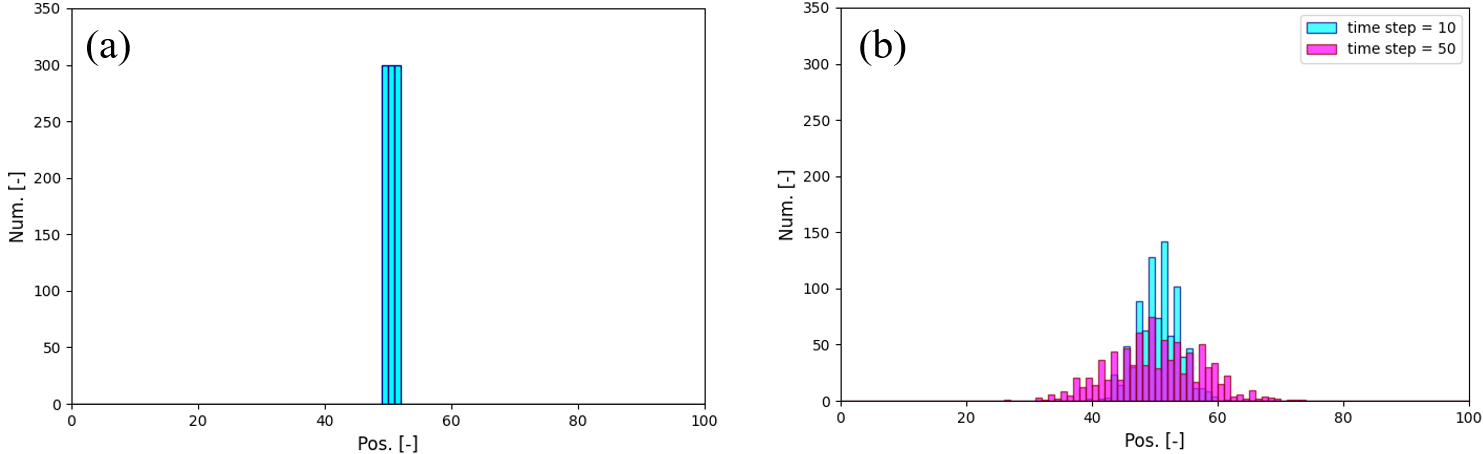
\includegraphics[width=14cm]{fig2.png}
\caption{ランダムウォークによる拡散現象のシミュレーション。(a)分子の初期分布(b)時間発展後の分子の分布。}
\end{center}
\end{figure}

\subsubsection{マクロな視点での物質拡散の解釈}

\begin{figure}[t]
\begin{center}
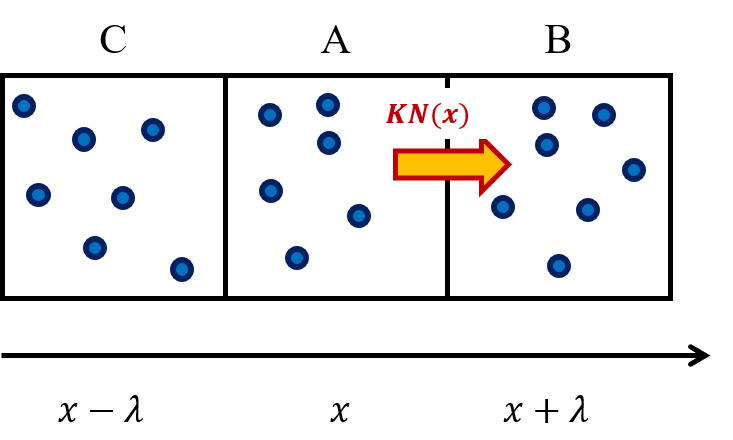
\includegraphics[width=8cm]{fig3.png}
\caption{局所分子数分布の概念図。}
\end{center}
\end{figure}

さて、本項ではマクロな視点に移動し、前述の議論から拡散項($D\Delta N$のようなもの)を導出できることを確認する。そこで、図3のような隣接した領域を設定しよう。図3の各領域は図1(a)のそれと同様である。ただし$D\Delta N$という形からも推測できるように、ここからは関数の微分を利用したい。つまり、粒子数の分布は滑らかな連続関数であって欲しいので各領域の幅$\lambda$は非常に小さいとする。一方で、各領域に含まれる分子数が少なくなる程$\lambda$を小さくしてしまえば、それはかえって関数の滑らかさを損なう。例えば領域$A$に分子が2個、領域$B$に分子が4個ある場合、$N(x)$と$N(x+\lambda)$で2倍の変化が生じる。逆に$A$に分子が1000個、$B$に分子が1002個ある場合、関数の滑らかさは先程より損なわれない。\par
つまり$\lambda$の値は「差分結果が微分と同様なぐらい小さく、各領域に十分な数の分子が存在するぐらい大きい」値がよい。これについて気体分子運動論では$\lambda$の値に平均自由行程を採用している。\par
本資料では、平均自由行程を「分子間の距離の平均値」と定義し、長さの単位を持つとする。これだけを聞くと平均的に見れば各領域に分子が1個だけ存在する訳で、関数の滑らかさを損なうように思われるかもしれない。しかしながら、平均自由工程はあくまで期待値であり、平均自由行程よりも短い距離にも分子は十分な数だけ存在する。\par
さて、先程「マクロに見たときの速度分布がゼロ」と仮定したが、これは各領域に含まれる分子に関する平均速度がゼロということであり、つまり分子は四方八方に等確率で移動していることに相当する(四方八方に等確率で進むという状態は正に残響音における音エネルギーの移動と類似する)。
従って、領域$A$から隣接領域へとランダムウォークによって移動する分子数に方向依存性はなく、単に$N(x)$に比例すると考えてよい。そこで、$A$から$B$へと単位時間に移動する分子数を$KN(x)$とする(ここで$K$は定数)。\par
$A$から$B$へと分子が移動するように、$B$から$A$へも分子が移動してくる。この量は同様に考えれば
\begin{equation}
KN(x+\lambda) \simeq KN(x)+K\partial_xN\left(x +\frac{\lambda}{2} \right)\lambda \notag
\end{equation}
となる(テイラー展開の1次の項まで考慮)。従って実質的に$A$から$B$への移動は右辺第二項の負の数だけ行われることになる。また、同様の計算を施すことで$A$から$C$へ移動する分子の数を計算できる。両者を纏めることで、$A$が単位時間あたりに放出する分子の数は
\begin{equation}
-D\partial_xN\left(x +\frac{\lambda}{2} \right) + D\partial_xN\left(x -\frac{\lambda}{2} \right) = \int_S -D \bm \nabla N \cdot \bm n dS
\end{equation}
となる($D=K\lambda$とした)。ここで$S=\{x-\lambda/2, x+\lambda/2 \}$は$A$の境界を表しており、最右辺は面積分を意味している。また$\bm n$は面要素$dS$に直交し、系外へと向く単位ベクトルである。上式の右辺はガウスの発散定理を用いることで、$\int_A -D\Delta NdV$と更に書き換えられる。この量の負値は単位時間当たりの領域$A$における分子増加数$\int_A \partial_tNdA$に相当するため、
\begin{equation}
\partial_t N= D\Delta N
\end{equation}
なる関係式が成立する。これが最も単純な拡散方程式である。ここまで1次元空間で議論してきたが、3次元になっても形は変わらない。\par
以上より、ランダムウォークで表現されていた拡散現象が、式(2)のような形に書き換えられると分かった。ただし物理的解釈としては式(1)の方が分かりやすいかもしれない。つまり、物理量にムラがあった場合、拡散現象はその勾配に比例する量の物質輸送を行う。その比例定数こそ正に拡散係数であり、平均自由行程に比例する。$-D\bm \nabla N \cdot \bm n$のような量を流束(flux)と言う。\par
ちなみに空間中で物質が湧き出す場合(臭気源など)、式(2)の拡散方程式にソース項$S$が加わり、$\partial_tN=D\Delta N+S$となる。また放射性物質のように対象の物質が消失する場合、減衰項と呼ばれるものが更に加わる。減衰項は$-\sigma N$のように表され、このときの支配方程式は
\begin{equation}
\partial_tN=D\Delta N-\sigma N+S
\end{equation}
となる。減衰項は振動工学におけるダンパーと類似の寄与を有する(ダンパーは速度に比例した反力を生み出し、物体の運動量を消失させていく)。なお、減衰項と拡散項の物理的解釈は明確にした方がようだろう。冒頭で、運動量保存則における拡散項は粘性応力だと述べた。一方の振動工学における減衰も液体の粘性などで生み出されている。どちらも流体の粘性を起因としている点で似ているが、拡散は図2のように局所的に高い物理量が減少しつつ周囲の物理量を増加させるのに対し、減衰は減少するのみである。つまり、物理量の輸送が見られるのが拡散であり、見られないのが減衰である。




\subsection{音響拡散方程式の直感的理解}
\subsubsection{Galton Boardの実験}

\begin{figure}[t]
\begin{center}
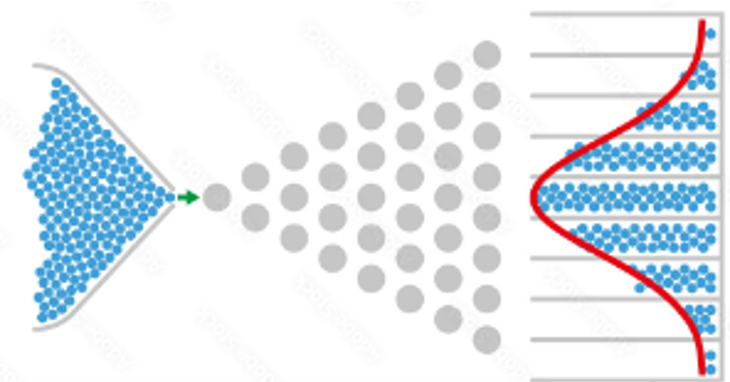
\includegraphics[width=8cm]{fig4.png}
\caption{Galton Boardの実験。}
\end{center}
\end{figure}

前節では1次元空間という単純な空間形状における分子の拡散を見てきた。分子の拡散が分子自身の熱的揺らぎやブラウン運動によって引き起こされていることは、図2の通りである。そのため拡散現象は拡散対象の分子が持つ特性とも言える。\par
しかしながら、実は空間形状が引き起こす疑似的な拡散というのも知られている。それを直感的に理解させてくれる例としてGalton Boardの実験を紹介しよう(Galton Boardの実験はYouTubeでも見られるので、是非検索してください)。\par
図4はGalton Boardの実験装置である。左側の小さな穴から青い粒子(分子やそれよりも巨視的な粒子であってもよい)が飛び出し、灰色の障害物にぶつかりながら右へと進んでいく。パチンコ玉のように、青い粒子は障害物(釘に相当)とぶつかるたびに進路を少し変える。その変化は確率的であるため、試行結果はその都度変わる。Galton Boardの実験が上手く制御されていれば、最終的に赤線のアンサンブル結果が得られる。\par
この実験結果は、局所的に分布していた物質が多項体にぶつかることでばらける現象を示している。もし青い粒子が光子であるならば、多項体による光の散乱と考えることもできるだろう。いずれにしても、多項体のようなものが存在することにより、図4中縦方向のバラつきが生まれることが分かる(横向きにもバラつきは生じるが、本資料では触れない)。\par
不確かさを無視すれば、多項体の存在は単なる境界条件に過ぎない。そのため、前節で見た分子同士の相互作用による拡散現象と、本実験で見られる現象は同様だと言えない。しかしながら、多項体と粒子の衝突という点が似ており、並びに多項体の微視的構造が分からないほどマクロに現象を観察している場合は本実験結果を拡散現象と同一視した方が都合よいといった点から、この現象をMechanical Dispersionと呼んでいる(日本語名は知らない。本資料では疑似拡散と呼ぶことにするが、完全に方言なので他では使わないこと)。\par

\begin{figure}[b]
\begin{center}
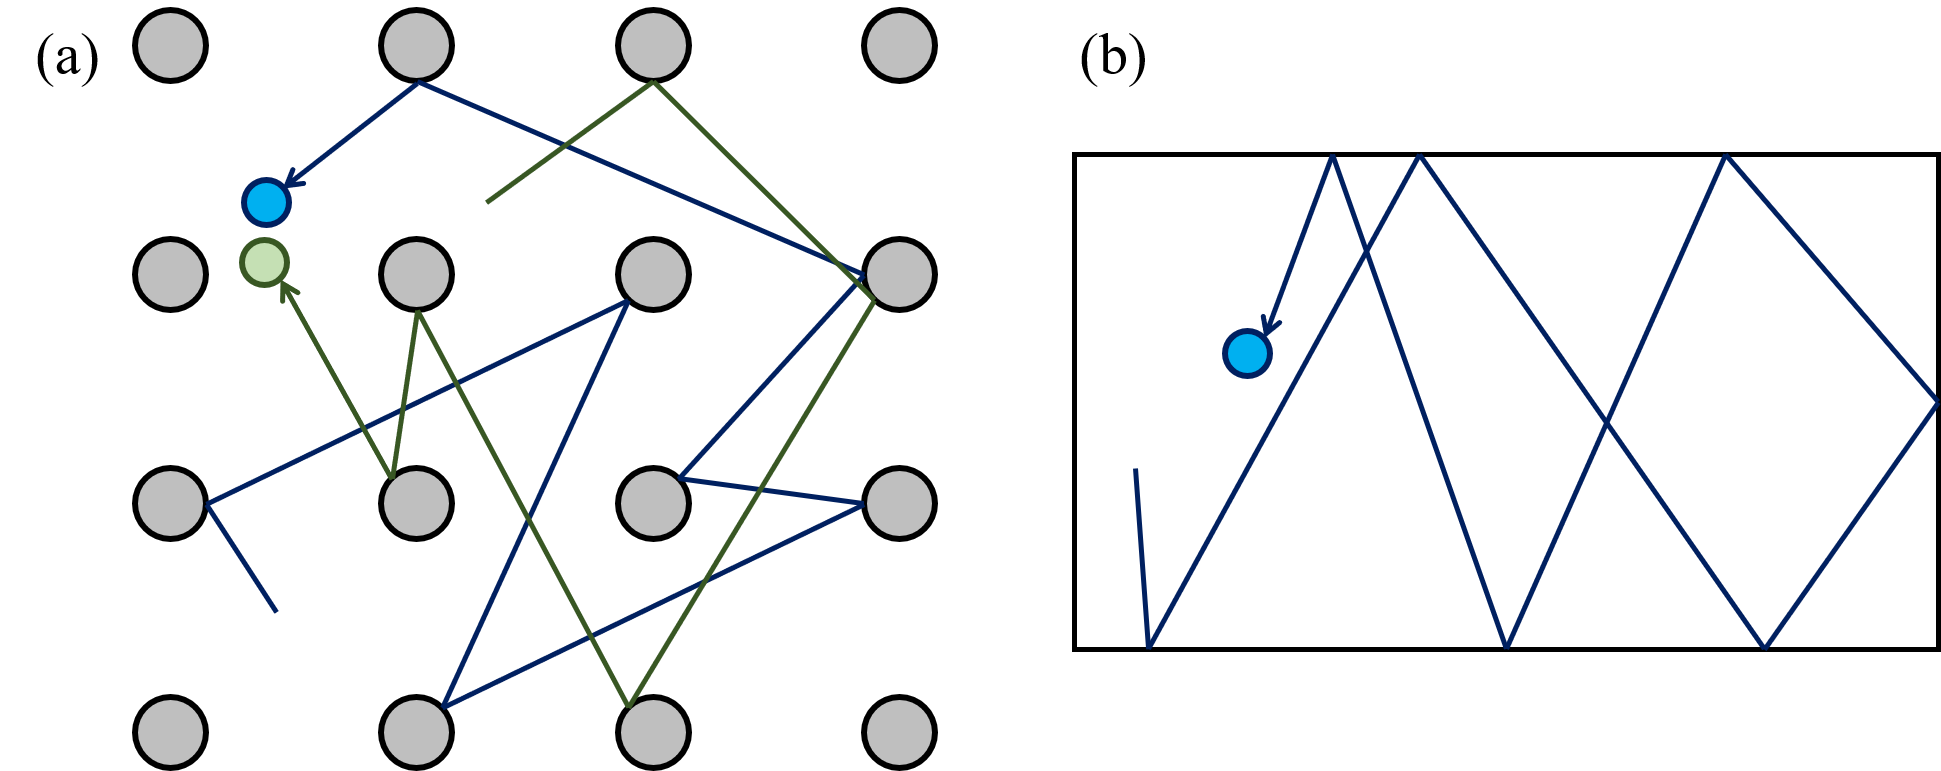
\includegraphics[width=10cm]{fig5.png}
\caption{疑似拡散と残響音の類似性。(a)多項体内での疑似拡散の様子(b)多重反射した音線の様子。}
\end{center}
\end{figure}

\subsubsection{音響拡散方程式の直感的理解}
疑似拡散現象は、Galton Boardの実験のように左から右への流れが無くても見られる。図5(a)は流のない多項体内におけるミクロな粒子(分子)などの運動を表している。前述の通り流れがなくとも熱的ゆらぎによりミクロな粒子は運動する。そして多孔体にぶつかる度に向きを変え、ブラウン運動のような動きを示す(もちろん粒子同士の衝突もあるので、従来の拡散もこの中では同時に生じている)。また、多数の粒子がブラウン運動しているので、図5(a)中の青色粒子と緑色粒子のように、近傍粒子が全く異なる向きに移動することもあり得る。つまり、疑似拡散によってマクロな流れが生じることはない。\par
このような多孔体内で生じる運動は、部屋空間における音線の軌跡と類似する(図5(b))。図5(b)のように、つまり幾何音響のように音エネルギーを有する仮想的な粒子の運動を考えたとき、残響音が支配的になっている頃には、多重反射した粒子の図5(a)のような運動が見られるだろう。したがって、物質拡散における分子は幾何音響における粒子に相当する(実際の幾何音響シミュレーションでは近似的にマクロな粒子を考えていると思うが)。そして粒子を沢山用意することで、図1(a)のような粒子のバラバラな動きを再現する。それらの統計量を抽出することで幾何音響は残響音に関する特性値を得る。この処理は多数の粒子を用意するという点で計算コストが高い。\par
一方で音響拡散方程式は分子のようなミクロな量を取り扱うのではなく、1.1.1項の$N(x)$のような分布関数を用いる。ただし音響拡散方程式の場合は音響エネルギー密度の分布関数とする(後述)。つまり、幾何音響よりもマクロな視点で捉え、多重反射の末に出来上がる粒子の無秩序な動きを拡散現象として考える訳である。マクロな視点な分、残響音に関する統計量を容易に求めることができるため、音響拡散方程式の計算コストは低いと言われている。

\section{音響拡散方程式の導出}
それでは本章より実際に音響拡散方程式を導出していく。これまでの議論を踏まえると、室内音響における壁の存在は多孔体の存在に相当することが分かる(図5)。当然ながら部屋の形状が変わると残響音の様子も変わるように、多項体の構造が変われば疑似拡散の様子も変わる。従ってまず初めに、部屋形状と多項体の対応を考えなければならない。\par
話を簡単にするために、本資料では半径$R$の多数の球で構成された多項体を考える。また、各球は図5(a)のように互いに接してなく、単位体積当たり$n_t$個の球が空間中に配置されているとする。このとき、単位体積当たりの多孔体の表面積は$4\pi R^2n_t$となる。\par
一方で、体積$V$かつ壁面総面積$S$の部屋空間を考える。この部屋における、単位体積当たりの壁面面積は$S/V$となる。従って多項体との対応関係より
\begin{equation}
4\pi R^2n_t=\frac{S}{V}
\end{equation}
が得られる。
\subsection{平均自由行程}
物質の拡散係数や流体の粘性係数は物性値として与えられることが多い。しかしながら、多項体内の疑似拡散に関する係数は決して物性値でなく、多項体の構造に依存する。1.1.1項で、拡散係数は平均自由行程に依存することを述べたが、疑似拡散においても同様である。そのため多項体内における平均自由行程の導出は重要である。\par
平均自由行程の定義は「分子間の距離の平均値」と前述したが、これは「ある粒子が衝突したのち、次に衝突するまでに進むことができる距離の期待値」と言い変えることができる。多項体の場合なら「衝突後に再度多項体に衝突するまでの距離の期待値」となるだろう。期待値という文言がある通り、平均自由行程には確率論的な考え方がある。そこで、衝突後に距離$x$だけ進んでも再衝突していない確率を$P(x)$とする。\par
$P(x)$に対して$P(x+dx)$は「$x$だけ進んでも衝突せず、かつ更に$dx$だけ進んでも衝突しない確率」と言える。いま、粒子の移動方向に垂直な単位面積の断面と、移動方向に長さ$dx$だけある直方体を考える。直方体の体積は$1 \times 1 \times dx$なため、この中には$n_tdx$個の球が存在する。粒子の移動方向に垂直な単位面積に対して、$n_tdx$個の球の投影面積は$\pi R^2n_t dx$となる(球を平面に投影すれば円になり、その面積は$\pi R^2$のため)。従って、$dx$だけ進むときに粒子が衝突しない確率は$1-\pi R^2 n_t dx$となる。以上より、$P(x+dx)=(1-\pi R^2 n_t dx)P(x)$なる関係が得られる。$P(x+dx)$をテイラー展開して1次の項まで考慮すれば$\partial_xP(x)=-\pi R^2 n_t P(x)$という微分方程式が得られる。定義より$P(0)=1$であるため、$P(x)$は$P(x)=\pi R^2 n_te^{-\pi R^2 n_t x}$と求めることができる。さて、平均自由工程$\lambda$は次にぶつかるまでの距離の期待値であったため、
\begin{equation}
\lambda=\int_0^\infty xP(x)dx=\frac{1}{\pi R^2 n_t}=\frac{4V}{S}
\end{equation}
と求まる(式(4)参照)。以上より、部屋空間に対応する多項体の平均自由工程が求められた。
\subsection{位置と速度に関するエネルギー密度関数}
音響拡散方程式ではマクロな視点で描像するため、図3のような系を考える。ただし粒子は流体粒子ではなく、音響エネルギーを有する仮想的な粒子とする。この点は幾何音響と同様と言えよう。各粒子が有する音響エネルギーは同じとみなし、音響エネルギーの分布は図3のように粒子の数密度で表される。例えば図3中の領域$A$には粒子が6個あるので、1個当たりの音響エネルギーを$W$としたとき、領域$A$の総音響エネルギーは$6W$となる。また、領域$A$の体積を$V_A$としたとき、音響エネルギー密度は$6W/V_A$となる。このように、1章では数密度の分布$N(x)$を考えていたが、それの代わりに音響エネルギー密度を考えても議論に差支えない。
これまで述べてきた通り、音響拡散方程式は音響エネルギー密度の分布を考え、「分布の勾配に比例した流束が生じる」という1章の結果もそのまま利用する。したがって、3次元空間のある点$\bm r$における、時刻$t$での流束(ベクトル)を$\bm J(\bm r, t)$と書き表したとき、音響エネルギー密度関数$w(\bm r, t)$との間に
\begin{equation}
\bm J(\bm r, t)=-D\bm \nabla w(\bm r, t)
\end{equation}
なる関係が成立する。ここで$D$は音響拡散方程式における拡散係数であり、後述の式(12)で求まる。\par
繰り返しになるが、音響エネルギー密度$w(\bm r, t)$は多数の粒子の空間平均値である。各粒子は壁面による多重反射を受けたため、同じ位置$\bm r$にいる粒子群でも、図1(a)のように移動する向きはバラバラである。そこで$w(\bm r, t)$のように、位置$\bm r$かつ時刻$t$において、速度$\bm v$を有する粒子を集め、それらによるエネルギー密度を$f(\bm r, \bm v, t)$とする。つまり、位置$\bm r$の領域に粒子が$N$個あったとき、$w(\bm r, t)=NW/V_A$だが、そのうち$N_v$個の粒子の速度だけが$\bm v$であるとき、$f(\bm r, \bm v, t)=N_vW/V_A$となる。これは位置(3次元)と速度(3次元)と時間(1次元)の関数なので、6次元の関数だと分かる(粒子の移動速度、つまり音速が一定であることを踏まえれば、$f$は5次元の関数と考えるべきである。しかし6次元であっても後の議論に支障をきたさないので、本資料では6次元のまま考える)。定義より、速度空間に関する積分
\begin{equation}
w(\bm r, t)= \iiint f(\bm r, \bm v, t) dV_v
\end{equation}
が得られる。ここで$dV_v$は$\bm v$に関する微小領域であり、$\bm r$に関する微小領域でない。また、3重積分は3つの速度成分に関する積分を意味する。

\subsection{壁面反射と吸音}

\begin{figure}[t]
\begin{center}
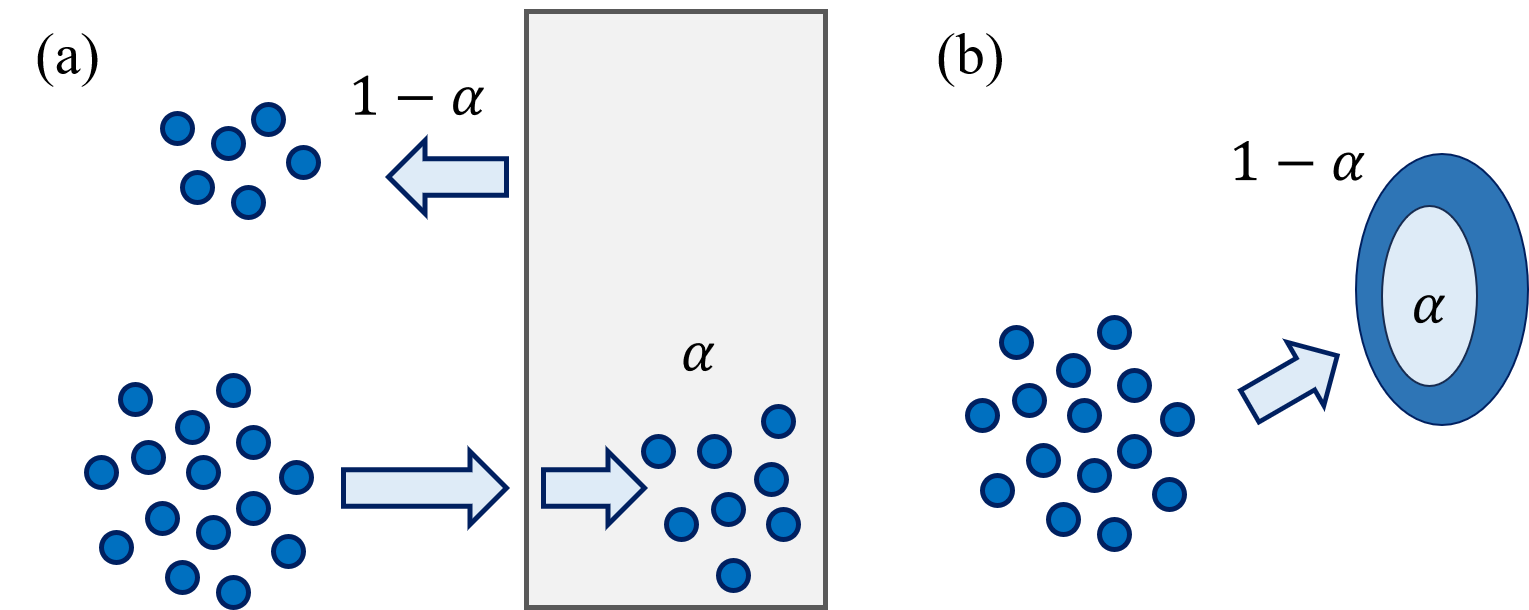
\includegraphics[width=10cm]{fig6.png}
\caption{壁面における反射と吸音の概念図。}
\end{center}
\end{figure}

1章の物質拡散では、粒子同士の衝突によるランダムウォークのみ考えてきた。なぜなら粒子同士が相互作用するとしたら、衝突しかないためである。また、Galton Boardの実験のような疑似拡散でも流体粒子と多項体の衝突のみを考えればよい。しかしながら、音響拡散方程式では衝突だけでなく吸音も生じるはずである。\par
吸音とは、波が境界に作用したときに起こる系外へのエネルギー輸送である。そのため吸音が発生したとき、その分だけ音響エネルギーが系内からなくなる訳で、これは音響エネルギーを有する仮想的な粒子の消失に相当する。したがって吸音が生じる室内音響の場合、支配方程式に減衰項が加わると想像できる(後述の式(13)参照)。\par
ところで吸音率とは入射してきた音響エネルギーに対する吸音された音響エネルギーの割合であるが、これは図6(a)のように解釈できる。つまり、$N$個の仮想的な粒子が壁面に衝突し、それぞれは確率$\alpha$で系内から消失し、確率$1-\alpha$で反射する。各粒子にとっては「消失するか反射するか」の2択に感じるが、$N$個の粒子で考えれば$\alpha$という実数値で表される割合の話になる。\par
多項体(もしくはそれに対応する室内空間)の吸音率が$\alpha$であったとする。時刻$t$のときに位置$\bm r$にいて、速度$\bm v$である粒子群$f(\bm r, \bm v, t)$を考えよう。当然ながらこの粒子たちは単位時間当たり$\bm v$だけ進む。この道中における、多項体の投影面積は単位面積当たり$\pi R^2n_t v$だけ占めることになる($v$は速度ベクトルのノルム)。従って$f(\bm r, \bm v, t)$の粒子群のうち$\pi R^2n_t vf(\bm r, \bm v, t)$だけ壁面と衝突することになる。このうち更に$\alpha\pi R^2n_t vf(\bm r, \bm v, t)$は吸音され、$(1-\alpha)\pi R^2n_t vf(\bm r, \bm v, t)$は反射する。\par
この議論から、吸音に関する別の解釈も生まれる。つまり、図6(b)のように多項体球の投影面積$Q_t = \pi R^2$のうち、$Q_a = \alpha \pi R^2$では吸音が必ず生じ、$Q_s=(1-\alpha)\pi R^2$では反射が必ず生じるというものである。粒子と多項体球のぶつかる位置が一様にランダムであれば、図6(b)の解釈でも確かに吸音率が$\alpha$になる(この解釈は音響拡散方程式の導出に重要であるが、本資料は多くの式展開を大胆に省いているため、この解釈を念頭にいれなくてもそれ程困らない)。
\subsection{音響拡散方程式の導出}
これまでに何度か述べてきたように、音響拡散方程式は音響エネルギー密度$w(\bm r, t)$に関する支配方程式である。ただし、その導出には位置と速度に関する音響エネルギー密度関数$f(\bm r, \bm v, t)$から始めなければならない。\par
$f(\bm r, \bm v, t)$に関する仮想粒子はその記載の通り速度$\bm v$に従って移動する。そのため多項体にぶつからない間、つまり仮想粒子の速度$\bm v$に変化が起きない間は
\begin{equation}
f(\bm r, \bm v, t)=f(\bm r+\bm vdt, \bm v, t+dt) \notag
\end{equation}
の関係を満たす。これをテイラー展開して2次以上の項を無視すると、
\begin{equation}
\partial_tf(\bm r, \bm v, t)=-\bm v \bm \nabla f(\bm r, \bm v, t) \notag
\end{equation}
なる関係を得る。なお、仮想粒子同士の衝突は無視してよい。仮想粒子同士の衝突は弾性衝突と考えてよく、それならば衝突によって起こる運動量や音響エネルギーの変化は、衝突相手の値との交換になる。各仮想粒子が有する音響エネルギーは同じとしているので、音響エネルギーの交換は実質的に無視できる。また運動量の交換も仮想粒子単位で見たの運動に影響を及ぼすかもしれないが、マクロに見た$f$の分布に影響を及ぼさない。したがって多項体への衝突のみ考える次第である。\par
上式は$f$に関する方程式の基礎であるが、ここから更に多項体の寄与を付加していく。まず、2.3節より多項体多項体は単位時間当たり$\alpha \pi R^2n_tvf(\bm r, \bm v, t)$の吸音と$(1-\alpha) \pi R^2n_tvf(\bm r, \bm v, t)$の反射を引き起こす。吸音が起きた場合、仮想粒子自体が消失するため$f$は減少する。反射の場合も速度ベクトル$\bm v$に変化が生じるため、結局$f$は減少する。よって、これら寄与を加えた新たな関係式
\begin{equation}
\partial_tf(\bm r, \bm v, t)=-\bm v \bm \nabla f(\bm r, \bm v, t)-\left\{\alpha \pi R^2 + (1-\alpha)\pi R^2 \right\}n_tvf(\bm r, \bm v, t)=-\bm v \bm \nabla f(\bm r, \bm v, t)-\pi R^2n_tvf(\bm r, \bm v, t) \notag
\end{equation}
が考えられる。更に、反射を受けて速度$\bm v'$から$\bm v$に変わった仮想粒子も考えなければならない。この場合は$f$を増加させるように働く。詳細な説明は省くが、この寄与は解析的に求めることが知られている。最終的に、$f$の支配方程式として
\begin{equation}
\partial_tf(\bm r, \bm v, t)=-\bm v \bm \nabla f(\bm r, \bm v, t)-\pi R^2n_tvf(\bm r, \bm v, t) + \frac{n_t\pi R^2 v}{4\pi}\iiint f(\bm r, \bm v', t)dV_{v'}
\end{equation}
が得られる。\par
さて、$w$と$f$には式(7)の関係があった。また式(8)の流束は位置$\bm r$で生じている平均的な流なので、
\begin{equation}
\bm J(\bm r, t)=\iiint \bm vf(\bm r, \bm v, t)dV_v \notag
\end{equation}
と書くこともできる(確率論における期待値の計算を想像)。音響拡散方程式は残響音に関するものだが、このときの仮想粒子の移動はバラついている(図5)。したがって$f$の$v$に対する依存は低い。そこで$f$を全速度方向に対する平均値$\bar f$と差分項$f'$に分け、$f=\bar f + f'$とする。残響音やランダムウォークのように、各位置で粒子の一様に進行する様子が見られる場合、$f'$の値は小さい。また音響拡散方程式における仮想粒子は全て音速の速さで進む(つまり速度ベクトルの向きは違えど大きさは同じ)。詳細な説明は省くが、以上を踏まえつつ速度に対する積分とテイラー展開を駆使すれば、
\begin{equation}
f(\bm r, \bm v, t) \simeq \frac{1}{4\pi}w(\bm r, t)+\frac{3}{4\pi v^2}\bm v \cdot \bm J(\bm r, t)
\end{equation}
なる関係を得る(ヒント:速度の大きさは一定なので、速度はデカルト座標$\bm v=(u, v, w)^{\rm T}$の代わりに球表面座標$(\theta, \phi)$で考えることができる。正に地球の緯度と経度に相等。半径1での球表面の表面積、つまり面積分結果は$4\pi$。式中の$4\pi$はここに由来する)。\par
式(9)を用いれば、式(8)は
\begin{equation}
\partial_t w+\frac{3}{v^2}\bm v \cdot \partial_t\bm J\simeq -\bm v \cdot \bm \nabla w-\frac{3}{v^2}\bm v \cdot \bm \nabla(\bm v \cdot \bm J)-\alpha \pi R^2 n_tvw-\frac{3}{v}\pi R^2n_t\bm v \cdot \bm J \notag
\end{equation}
のように書き換えられる。
ただし残響音やランダムウォークのように、マクロに見れば一様に進行している問題の場合、$\bm J$の時間微分は小さいと考え、左辺第2項は無視できる。また、式(6)より右辺第1項と第4項には等式が成立することが想像できる。したがって上式を
\begin{equation}
\left\{
\begin{array}{l}
\bm J \simeq -\frac{v}{3\pi R^2 n_t}\bm \nabla w \\
\partial_t w \simeq -\frac{3}{v^2}\bm v \cdot \bm \nabla(\bm v \cdot \bm J)-\alpha \pi R^2 n_tvw
\end{array}\right.
\end{equation}
のように分割することにしよう。\par
式(10)の1つ目の式は式(5)より
\begin{equation}
\bm J \simeq -\frac{\lambda v}{3}\bm \nabla w=-\frac{4Vv}{3S}\bm \nabla w
\end{equation}
と書き直すことができる。ここで$v$は仮想粒子の速さなので、音速を代入すればよい。この式は流束と音響エネルギー密度勾配の関係であることから、係数
\begin{equation}
D=\frac{4Vv}{3S}
\end{equation}
は拡散係数に相当することが分かる。したがって音響拡散方程式における拡散係数は部屋形状のみから求められるようになった。\par
式(10)の2つ目の式に式(11)を代入することで、
\begin{equation}
\partial_t w=D\Delta w-\sigma w
\end{equation}
なる関係式を得る。ここで$\sigma = (\alpha Sv)/(4V)$であり、右辺第二項は吸音による寄与を意味する(減衰項)。そして式(11)こそが正に音響拡散方程式と呼ばれるものである。空間中に音源がある場合は、式(13)にソース項を加えたもの
\begin{equation}
\partial_t w=D\Delta w-\sigma w+P
\end{equation}
を考える。因みに$P$は単位時間当たりに生成される音響エネルギー密度なので、音響パワーの空間密度分布と解釈できる。


\subsection{吸音と境界条件について}
本来吸音は部屋の境界部分で生じるはずだが、音響拡散方程式では式(14)のように部屋全体で起きていると考える。これは部屋という空間を多項体で模擬したためである。また音響拡散方程式を数値解析する場合、境界条件にはノイマン境界条件
\begin{equation}
\bm n \cdot \bm \nabla w=0
\end{equation}
を用いる。ここで$\bm n$は境界に垂直な方向のベクトルである。ノイマン境界条件を採用する意図としては、吸音以外の理由でエネルギーが消失させないことにある。流束が音響エネルギー密度の勾配に比例することは前述の通りで、もしも式(15)が成立するなら、拡散による音響エネルギーの漏洩が防止される。
\subsubsection{音響拡散方程式の別の形式}
式(14)及び式(15)による数値解析は音響拡散方程式の一般的な手法の一つだが、空間全体に吸音の寄与を持たせることと、辻褄を合わせるような境界条件の設定には否定的な意見も存在する。例えば実際の部屋を考える場合、境界と一言で聞いてもそれにはソファやテーブル、キッチンなど様々であり、吸音率の値もその数だけある。このような問題に対して、どのような吸音率の値を空間に与えればよいだろうか。直感的に、ソファ周辺の空間にはソファの吸音率を与えればよさそうだが、周辺の定義があいまいである。そのため実際のシミュレーションでは、部屋全体の境界を加味して便宜的な吸音率を計算し、それを部屋全体に与えることが多い。この方法だと実装が容易になるが、やはり厳密さを欠く。そのため、いまでは空間に吸音の機能を与えず壁面にのみ与える手法が提案されている。\par
吸音の寄与を境界でのみ起こしたい場合は、支配方程式から減衰項を取り除き、境界条件にロビンの境界条件を採用すればよい。つまり、
\begin{equation}
\partial_tw=D\Delta w+P
\end{equation}
なる支配方程式と
\begin{equation}
-D\bm n \cdot \bm \nabla w =\frac{v\alpha}{4}
\end{equation}
なる境界条件を考える。複雑な境界条件を有する問題の場合は、式(16)(17)を用いることが多い。

\end{document}




















